\definecolor{bgLight}{HTML}{F8FAFC}
\definecolor{lvlRootBg}{HTML}{4f6fb9}
\definecolor{lvlRootText}{HTML}{F8FAFC}
\definecolor{lvlRootBorder}{HTML}{0284C7}
\definecolor{lvlSectorFill}{HTML}{E0F2FE}
\definecolor{lvlSectorBorder}{HTML}{0284C7}
\definecolor{lvlSectorText}{HTML}{0369A1}
\definecolor{lvlRoleFill}{HTML}{F1F5F9}
\definecolor{lvlRoleBorder}{HTML}{475569}
\definecolor{lvlRoleText}{HTML}{1E293B}
\definecolor{lvlToolFill}{HTML}{CCFBF1}
\definecolor{lvlToolBorder}{HTML}{0D9488}
\definecolor{lvlToolText}{HTML}{0F766E}
\pgfdeclarelayer{bg}
\pgfsetlayers{bg,main}

\newcommand{\nd}[4]{%
  \node[
    draw=#4Border,
    fill=#4Fill,
    text=#4Text,
    line width=1.1pt,
    rounded corners=6pt,
    inner sep=6pt,
    align=center,
    font=\sffamily\bfseries\footnotesize
  ] (#1) at (#2) {#3};%
}

\newcommand{\conn}[5]{%
  \draw[#1Border, line width=#5pt, line cap=round, opacity=0.65] (#2) -- (#3);%
}

\begin{multicols*}{2}
\inicializarSeccion{Introducción}

\begin{center}
  \includesvg[width=0.8\linewidth]{fase1/SDG9.svg}
  \captionof{figure}{ODS \#9: Industria, innovación e infraestructura.}
  \label{fig:introduccion}
\end{center}

En esta sección, hablaremos acerca de los Objetivos de Desarrollo Sostenible de las Naciones Unidas. Especificamente, del ODS \#9, que se enfoca en la industria, innovación e infraestructura. La motivación de esta decisión se basa a las personas que nosotros queremos apoyar con nuestro proyecto. Queremos apoyar al sector industrial con el manejo de herramientas y materiales, así como a los trabajadores técnicos que se encargan de la operación del dia a día de la industria.

\end{multicols*}
% Diagrama de ODS 9
\begin{center}
\resizebox{\textwidth}{!}{%
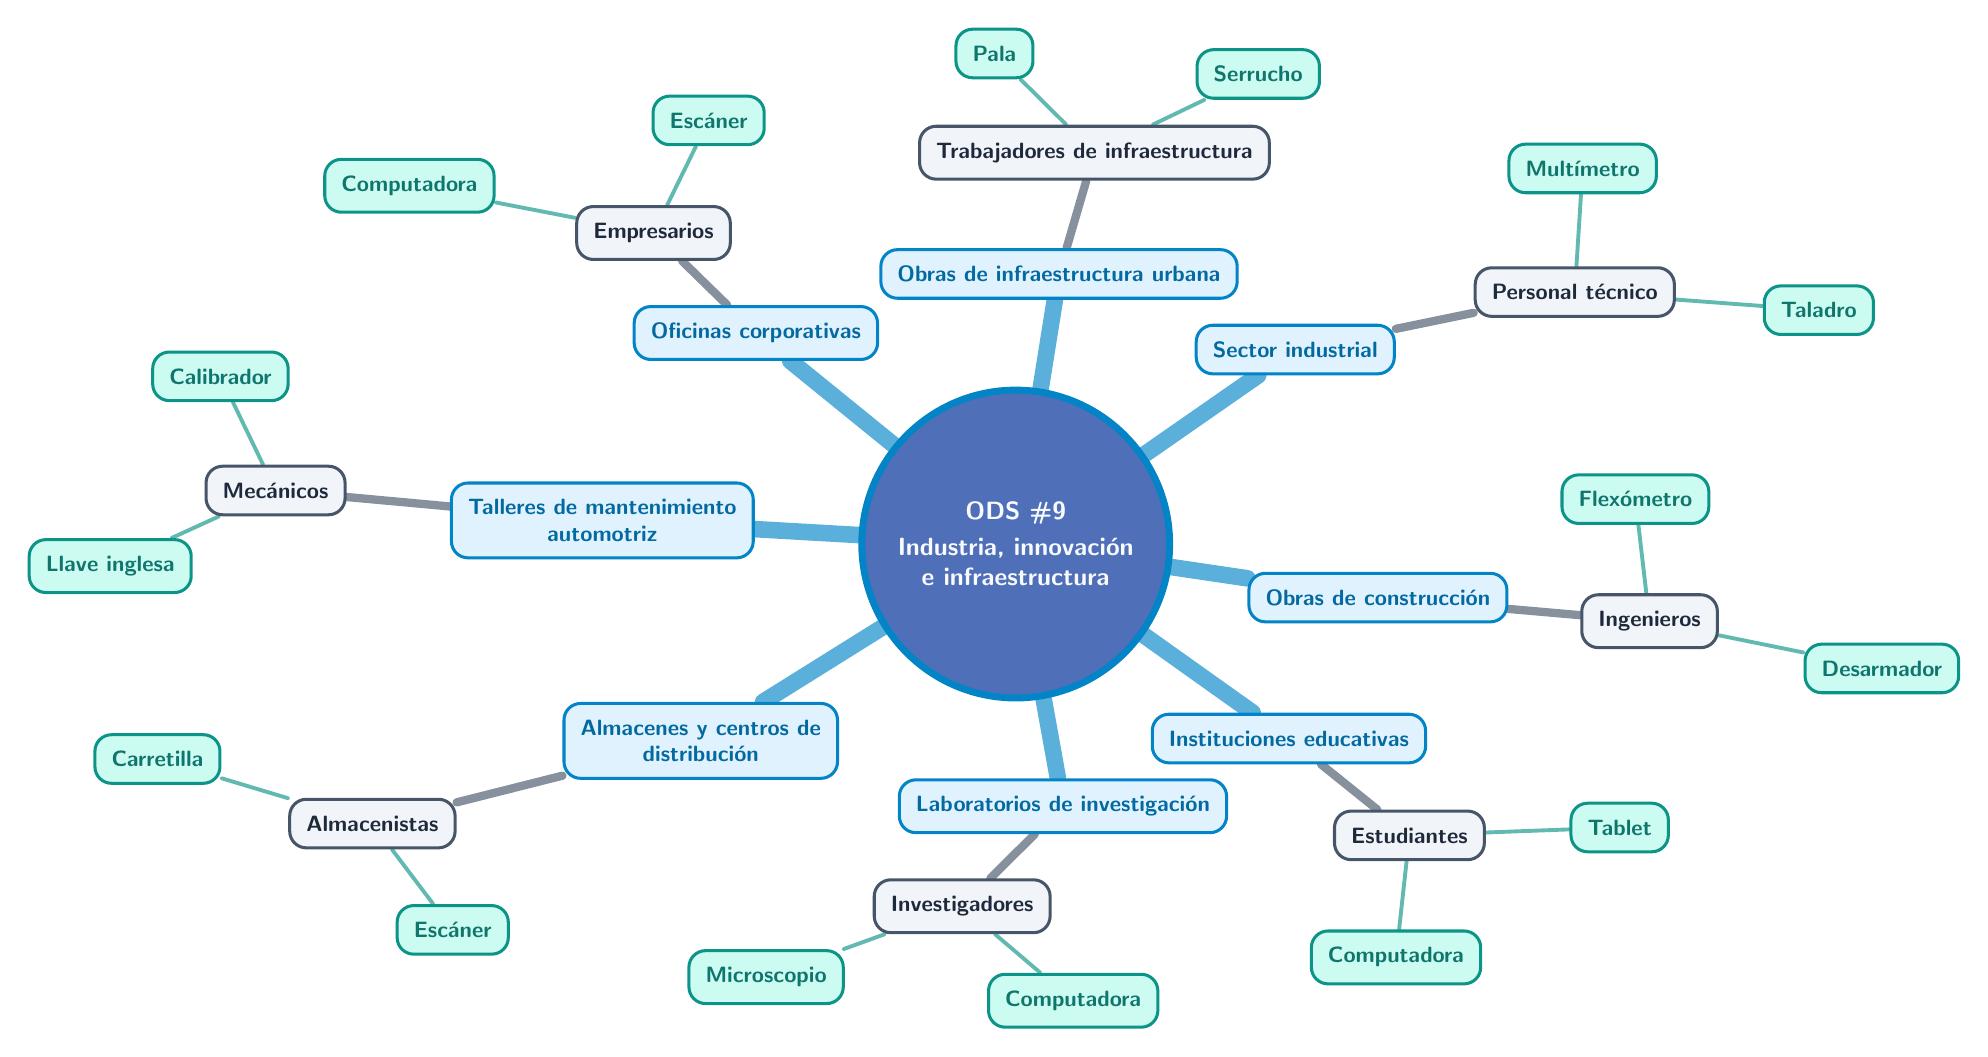
\begin{tikzpicture}[
  root/.style={
    circle,
    fill=lvlRootBg,
    draw=lvlRootBorder,
    line width=2.5pt,
    text=lvlRootText,
    align=center,
    font=\sffamily\bfseries\small,
    inner sep=8pt
  }
]

\node[root] (R) at (0,0) {\textbf{ODS \#9}\\[2pt] Industria, innovación\\e infraestructura};
\nd{s1}{3.55,2.47}{Sector industrial}{lvlSector}
\nd{s2}{7.1,3.2}{Personal técnico}{lvlRole}
\nd{s3}{7.2,4.77}{Multímetro}{lvlTool}
\nd{s4}{10.2,2.97}{Taladro}{lvlTool}
\nd{c1}{4.6,-0.68}{Obras de construcción}{lvlSector}
\nd{c2}{8.05,-0.98}{Ingenieros}{lvlRole}
\nd{c3}{7.87,0.57}{Flexómetro}{lvlTool}
\nd{c4}{11,-1.58}{Desarmador}{lvlTool}
\nd{e1}{3.47,-2.47}{Instituciones educativas}{lvlSector}
\nd{e2}{5,-3.7}{Estudiantes}{lvlRole}
\nd{e3}{7.67,-3.6}{Tablet}{lvlTool}
\nd{e4}{4.83,-5.25}{Computadora}{lvlTool}
\nd{l1}{0.6,-3.33}{Laboratorios de investigación}{lvlSector}
\nd{l2}{-0.68,-4.6}{Investigadores}{lvlRole}
\nd{l3}{-3.17,-5.5}{Microscopio}{lvlTool}
\nd{l4}{0.73,-5.8}{Computadora}{lvlTool}
\nd{a1}{-4,-2.5}{Almacenes y centros de\\distribución}{lvlSector}
\nd{a2}{-8.17,-3.55}{Almacenistas}{lvlRole}
\nd{a3}{-10.9,-2.73}{Carretilla}{lvlTool}
\nd{a4}{-7.15,-4.9}{Escáner}{lvlTool}
\nd{t1}{-5.25,0.3}{Talleres de mantenimiento\\automotriz}{lvlSector}
\nd{t2}{-9.4,0.68}{Mecánicos}{lvlRole}
\nd{t3}{-10.1,2.13}{Calibrador}{lvlTool}
\nd{t4}{-11.5,-0.28}{Llave inglesa}{lvlTool}
\nd{o1}{-3.3,2.68}{Oficinas corporativas}{lvlSector}
\nd{o2}{-4.6,3.95}{Empresarios}{lvlRole}
\nd{o3}{-7.7,4.55}{Computadora}{lvlTool}
\nd{o4}{-3.9,5.38}{Escáner}{lvlTool}
\nd{u1}{0.55,3.43}{Obras de infraestructura urbana}{lvlSector}
\nd{u2}{1.0,4.97}{Trabajadores de infraestructura}{lvlRole}
\nd{u3}{-0.27,6.23}{Pala}{lvlTool}
\nd{u4}{3.08,5.97}{Serrucho}{lvlTool}
\begin{pgfonlayer}{bg}
  \foreach \p in {s,c,e,l,a,t,o,u}{
    \conn{lvlSector}{R}{\p1}{}{6}
    \conn{lvlRole}{\p1}{\p2}{}{3}
    \conn{lvlTool}{\p2}{\p3}{}{1.4}
    \conn{lvlTool}{\p2}{\p4}{}{1.4}
  }
\end{pgfonlayer}

\end{tikzpicture}%
}
\end{center}